\section{Backend}
\subsection{Descrizione generale}\label{beDescrizione}
Le funzionalità previste dalla piattaforma hanno permesso di individuare i seguenti domini:
\begin{itemize}
	\item \textbf{Products;}
	\item \textbf{Categories;}
	\item \textbf{Payments;}
	\item \textbf{Orders;}
	\item \textbf{Cart;}
	\item \textbf{Addresses;}
	\item \textbf{Users.}
\end{itemize}
I domini sono stati uniti riflettendo sulle loro interdipendenze al fine di individuare dei \glo{microservizi} utili per procedere con lo sviluppo, in particolare sono stati identificati i microservizi:
\begin{itemize}
	\item \textbf{Products-categories service;}
	\item \textbf{Payments-orders service;}
	\item \textbf{Carts service;}
	\item \textbf{Addresses service;}
	\item \textbf{Users service.}
\end{itemize}
Lo sviluppo di singoli servizi permette una maggiore possibilità di sviluppo in parallelo dei singoli domini grazie alla loro struttura e all'agilità degli aggiornamenti e la possibilità di gestire i dati in modo decentralizzato.

\subsection{Struttura dei microservizi}\label{StrutturaMicroservizi}
\begin{figure}[H]
	\centering
	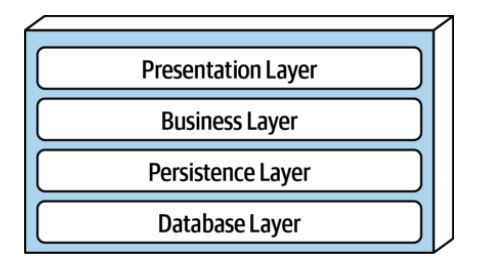
\includegraphics[scale=0.4]{Immagini/Backend/layer.png}
	\caption{layered architecture}
	\label{fig:layer}
\end{figure}
La struttura di ogni singolo servizio si basa su una \textbf{layered architecture} dove i componenti sono organizzati in vari strati che comunicano tra loro, il principale vantaggio è che risulta molto più semplice procedere ai test attraverso \glo{mock}.\\
Andando ad analizzare il singolo microservizio abbiamo:
\begin{center}
	\begin{minipage}{0.3\textwidth}
		\centering
		
\includegraphics[scale=0.78]{Immagini/Backend/Amazon-DynamoDB.png}
		\captionof{figure}{DynamoDB}
	\end{minipage}
	\begin{minipage}{0.3\textwidth}
		\centering
		
\includegraphics[scale=0.19]{Immagini/Backend/AWSLambda.png}
		\captionof{figure}{Lambda}
	\end{minipage}
	\begin{minipage}{0.3\textwidth}
		\centering
		
\includegraphics[scale=0.26]{Immagini/Backend/Gateway.png}
		\captionof{figure}{API Gateway}
	\end{minipage}
\end{center}
\begin{itemize}
	\item \textbf{DynamoDB:} per gestire i vari dati;
	\item \textbf{Lambda:} le funzioni che lavorano sui dati del database;
	\item \textbf{API Gateway:} riceve e gestisce le richieste del client richiamando le lambda e restituendone i risultati.
\end{itemize}

\subsubsection{Products-categories service}
\begin{figure}[H]
	\centering
	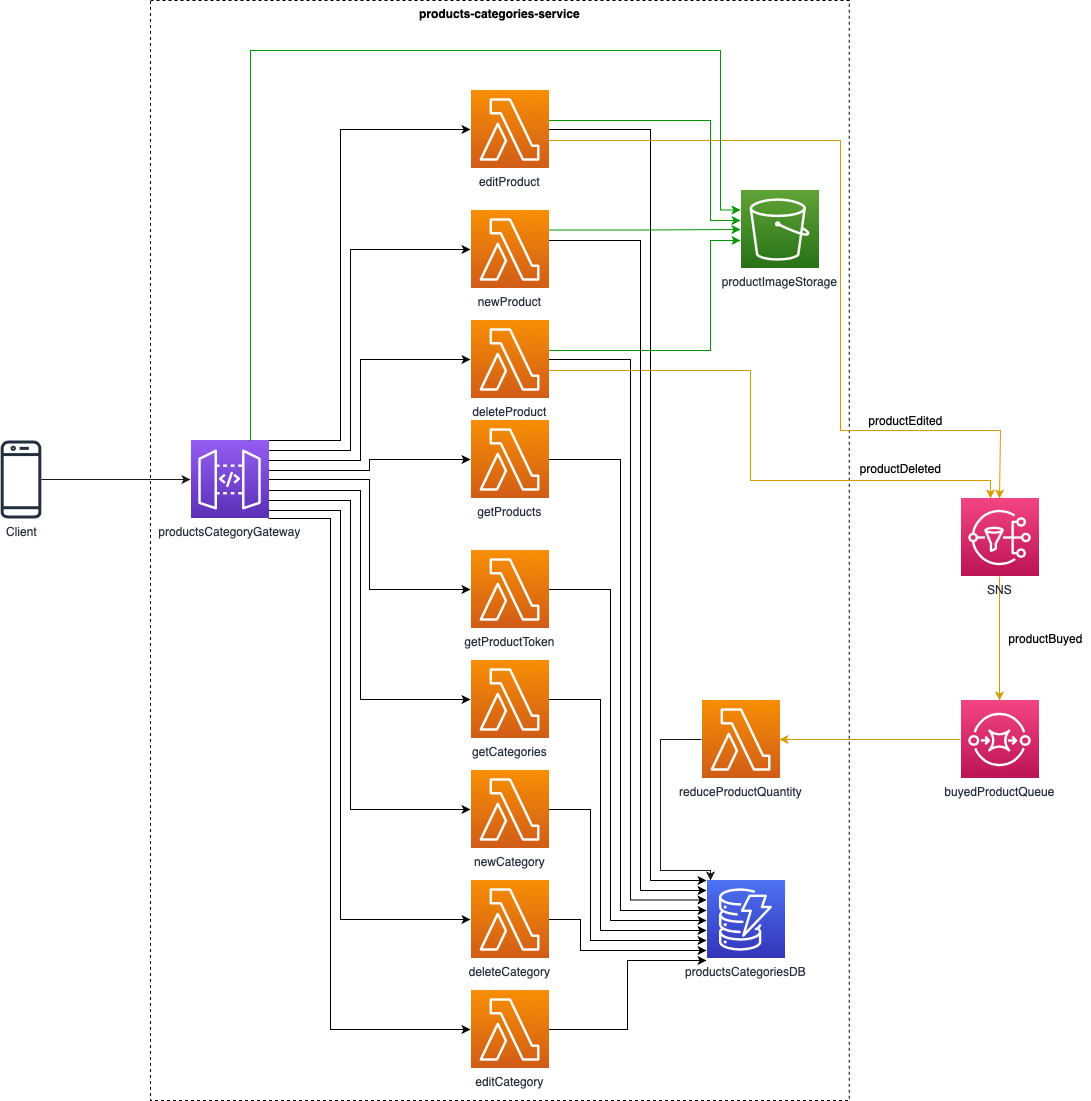
\includegraphics[scale=0.4]{Immagini/Backend/AWSProductsCategories.png}
	\caption{Products-categories service}
	\label{fig:ProductCategories}
\end{figure}
Il microservizio \textbf{products-categories} fornisce le principali funzionalità per gestire i prodotti e le categorie alle quali vengono assegnati per le funzioni di ricerca. Sono esempi di funzioni usufruibili dall'utente:
\begin{itemize}
	\item Inserimento di un nuovo prodotto;
	\item Eliminazione di un prodotto già presente nella piattaforma;
	\item Modifica delle specifiche di un prodotto;
	\item Inserimento di una nuova categoria per la classificazione dei vari prodotti in vendita.
\end{itemize}\noindent
Oltre all'utilizzo come per i successivi microservizi di AWS API Gateway, AWS Lambda e AWS DynamoDB viene impiegato Amazon S3 bucket per gestire le immagini associate ad un prodotto e Amazon SNS e SQS permettono il controllo della modifica/eliminazione di un prodotto assicurando la corretta validità della quantità disponibile dello stesso.

\subsubsection{Payments-orders service}
\begin{figure}[H]
	\centering
	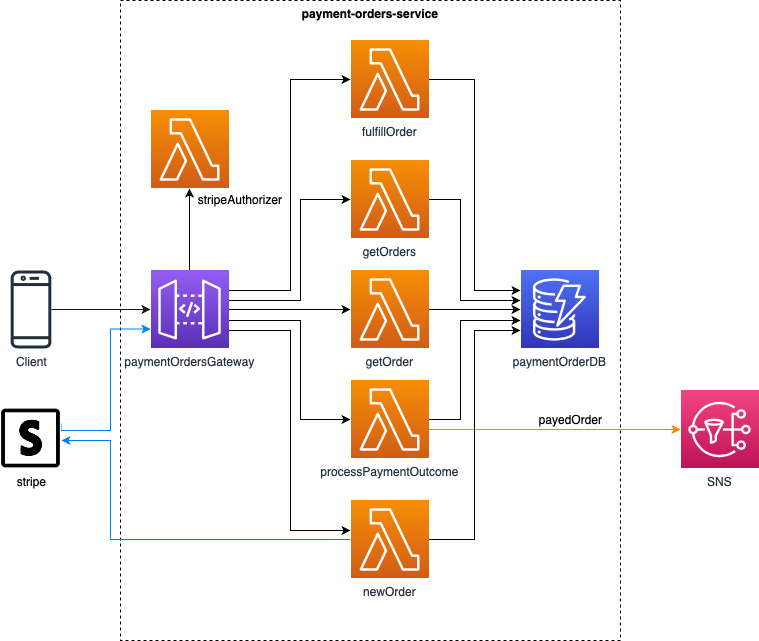
\includegraphics[scale=0.4]{Immagini/Backend/AWSPaymentOrders.png}
	\caption{Payments-orders service}
	\label{fig:Payment-orders}
\end{figure}
Il microservizio \textbf{payments-orders} fornisce le principali funzionalità per gestire il pagamento di un ordine e garantire la storicizzazione degli ordini effettuati. Anche in questo microservizio viene utilizzato Amazon SNS per assicurare il corretto risultato del pagamento, gestito dal servizio esterno Stripe.

\subsubsection{Carts service}
\begin{figure}[H]
	\centering
	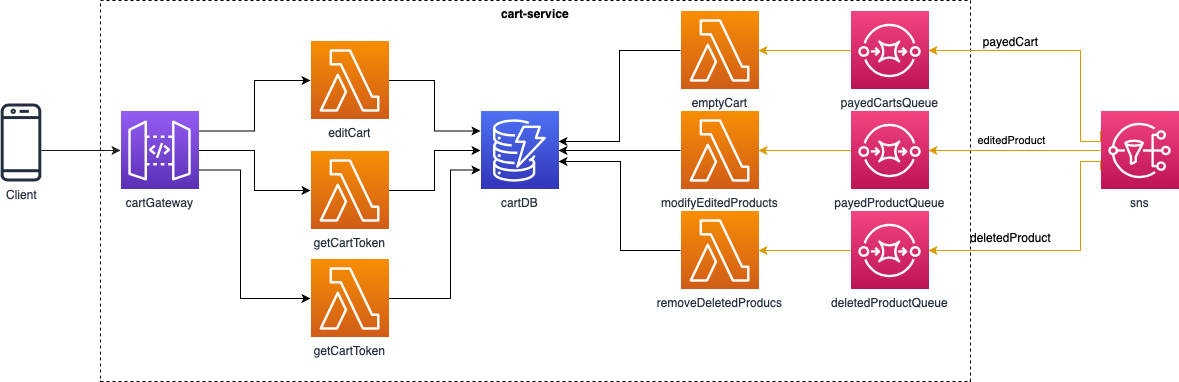
\includegraphics[scale=0.4]{Immagini/Backend/AWSCart.png}
	\caption{Carts service}
	\label{fig:Cart}
\end{figure}
Il microservizio \textbf{carts} fornisce le principali funzionalità per gestire il carrello dell'utente assicurando che eventuali modifiche fatte sui suoi prodotti esternamente, ad esempio il venditore modifica il prezzo di un prodotto, si riflettano anche all'interno dei carrelli degli utenti attraverso l'utilizzo di Amazon SNS e SQS.

\subsubsection{Addresses service}
\begin{figure}[H]
	\centering
	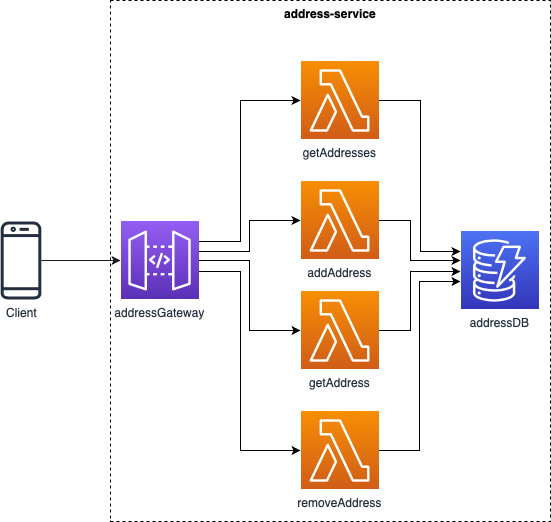
\includegraphics[scale=0.4]{Immagini/Backend/AWSAddresses.png}
	\caption{Addresses service}
	\label{fig:Adresses}
\end{figure}
Il microservizio \textbf{addresses} fornisce le principali funzionalità per gestire gli indirizzi di spedizione di un utente come l'aggiunta o la rimozione di un indirizzo. In questo microservizio entrano in gioco solo AWS API Gateway, AWS Lambda e AWS DynamoDB.

\subsubsection{Users service}
\begin{figure}[H]
	\centering
	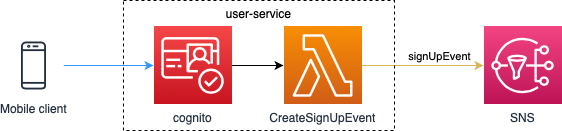
\includegraphics[scale=0.7]{Immagini/Backend/AWSUserService.png}
	\caption{Users service}
	\label{fig:Users}
\end{figure} 
Il microservizio \textbf{users} fornisce le principali funzionalità per gestire la registrazione e l'autenticazione di un utente alla piattaforma attraverso l'utilizzo di AWS Cognito.

\subsection{Struttura del backend}\label{Strutturabe}
\begin{figure}[H]
	\centering
	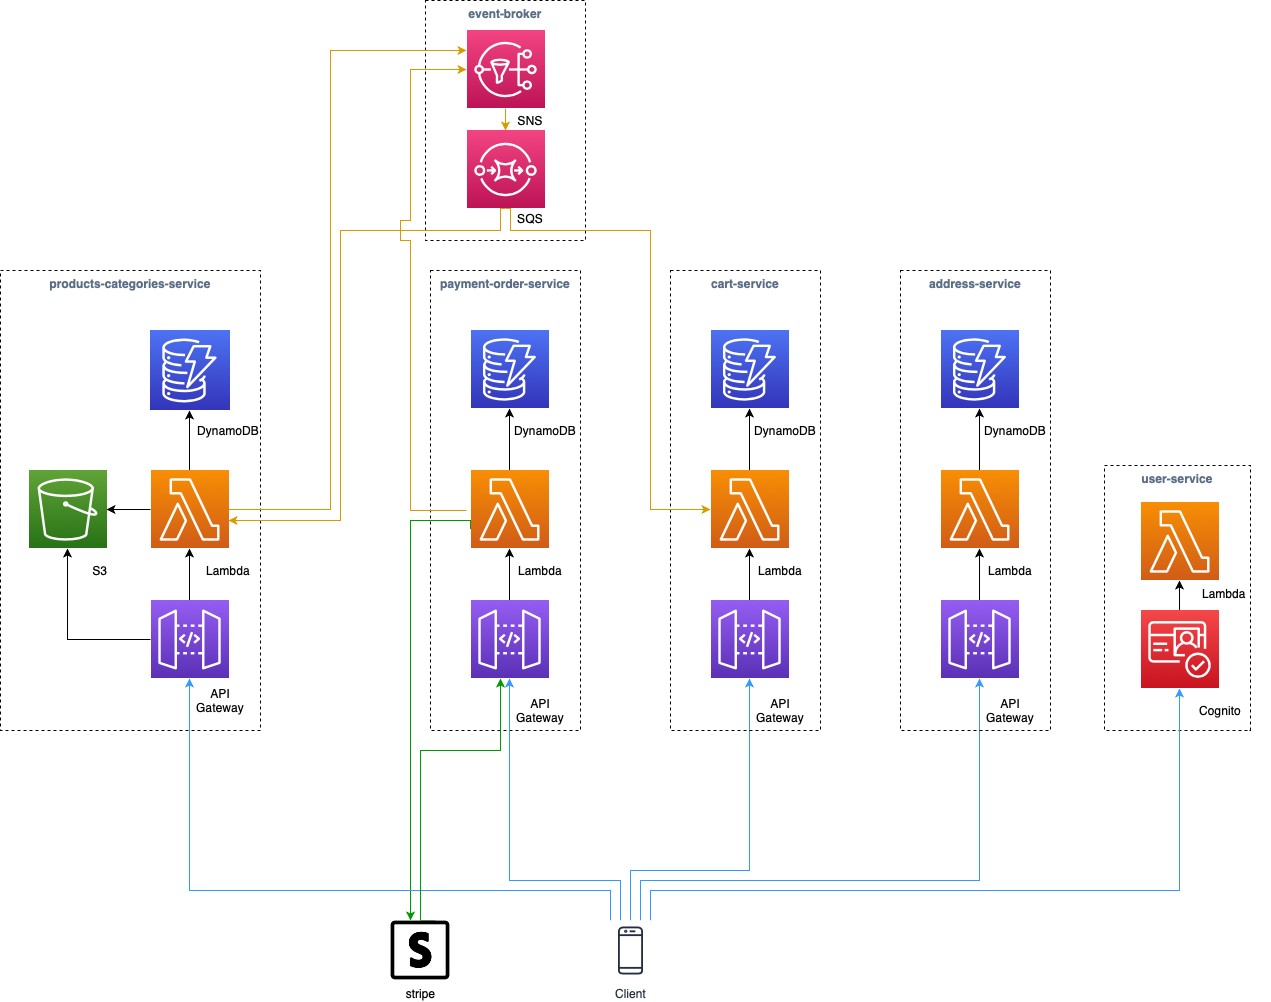
\includegraphics[scale=0.4]{Immagini/Backend/AWSArchitecture.png}
	\caption{Architettura backend}
	\label{fig:backend}
\end{figure}
Per slegare i microservizi tra di loro vengono utilizzate due strategie. La prima consiste nel gestire le chiamate asincrone attraverso SNS il servizio che fa da \glo{event broker} su AWS, eliminando così lo sviluppo di integrazioni tra microservizi e limitandosi a quelle per il \glo{message broker}.
La seconda invece è pensata per eliminare le chiamate sincrone tra microservizi, come quelle di validazione. Per far ciò si utilizza la firma digitale legata a un microservizio per verificare l'integrità delle richieste del client, sostituendo così le varie integrazioni necessarie a un semplice check attraverso la chiave pubblica del microservizio.

\subsection{Diagrammi di sequenza}\label{Diagrammiseq}
Di seguito sono riportati i diagrammi di sequenza per descrivere alcune delle principali operazioni effettuabili all'interno della piattaforma.
\subsubsection{Creazione ed eliminazione di un prodotto effettuata dal venditore}
\begin{figure}[H]
	\centering
	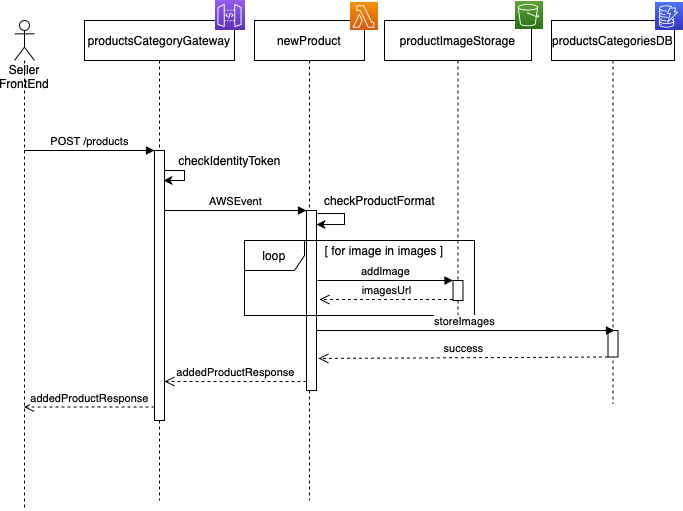
\includegraphics[scale=0.5]{Immagini/Backend/CreazioneProdotto.png}
	\caption{Creazione di un nuovo prodotto nella piattaforma}
	\label{fig:DiagrammaCreazioneProdotto}
\end{figure}
\begin{figure}[H]
	\centering
	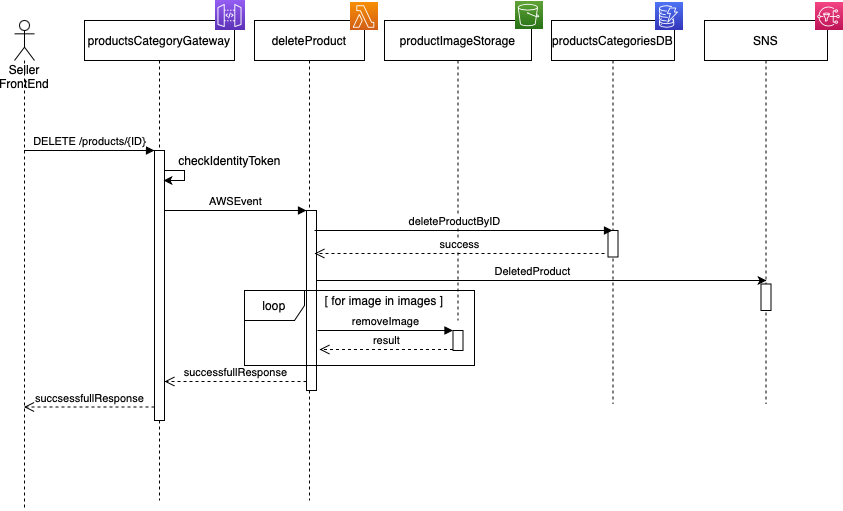
\includegraphics[scale=0.47]{Immagini/Backend/EliminazioneProdotto.png}
	\caption{Eliminazione di un prodotto dalla piattaforma}
	\label{fig:DiagrammiEliminazioneProdotto}
\end{figure}
I diagrammi rappresentano rispettivamente la creazione e l'eliminazione di un prodotto dalla piattaforma, in queste operazioni è necessario prevedere la gestione del salvataggio delle eventuali immagini associate ai prodotti tramite Amazon S3 bucket.
\subsubsection{Aggiunta di un prodotto al carrello}
\begin{figure}[H]
	\centering
	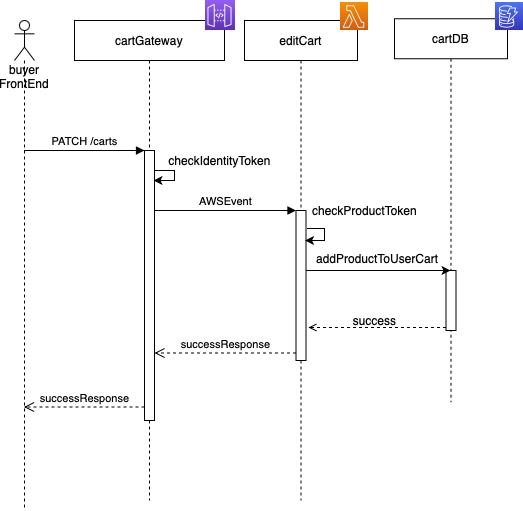
\includegraphics[scale=0.5]{Immagini/Backend/AggiuntaProdottoAlCarrello.png}
	\caption{Aggiunta di un prodotto al carrello}
	\label{fig:DiagrammaCarrello}
\end{figure}
Il diagramma rappresenta l'interazione delle tecnologie quando l'utente aggiunge un nuovo prodotto al carrello, in questo caso occorre modificare lo stato del carrello.
\subsubsection{Modifica di un indirizzo di spedizione}
\begin{figure}[H]
	\centering
	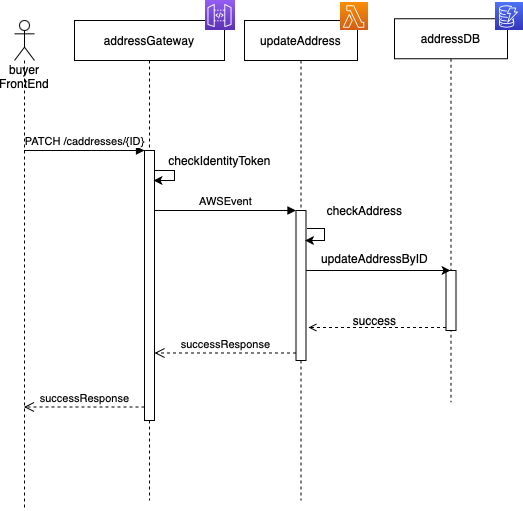
\includegraphics[scale=0.5]{Immagini/Backend/ModificaIndirizzo.png}
	\caption{Modifica di un indirizzo di spedizione}
	\label{fig:DiagrammaModificaindirizzo}
\end{figure}
All'interno della piattaforma l'acquirente può aggiungere, eliminare o modificare gli indirizzi di spedizione inseriti, il diagramma rappresenta la collaborazione delle tecnologie per effettuare quest'ultima operazione.
\subsubsection{Pagamento e creazione di un ordine}
\begin{figure}[H]
	\centering
	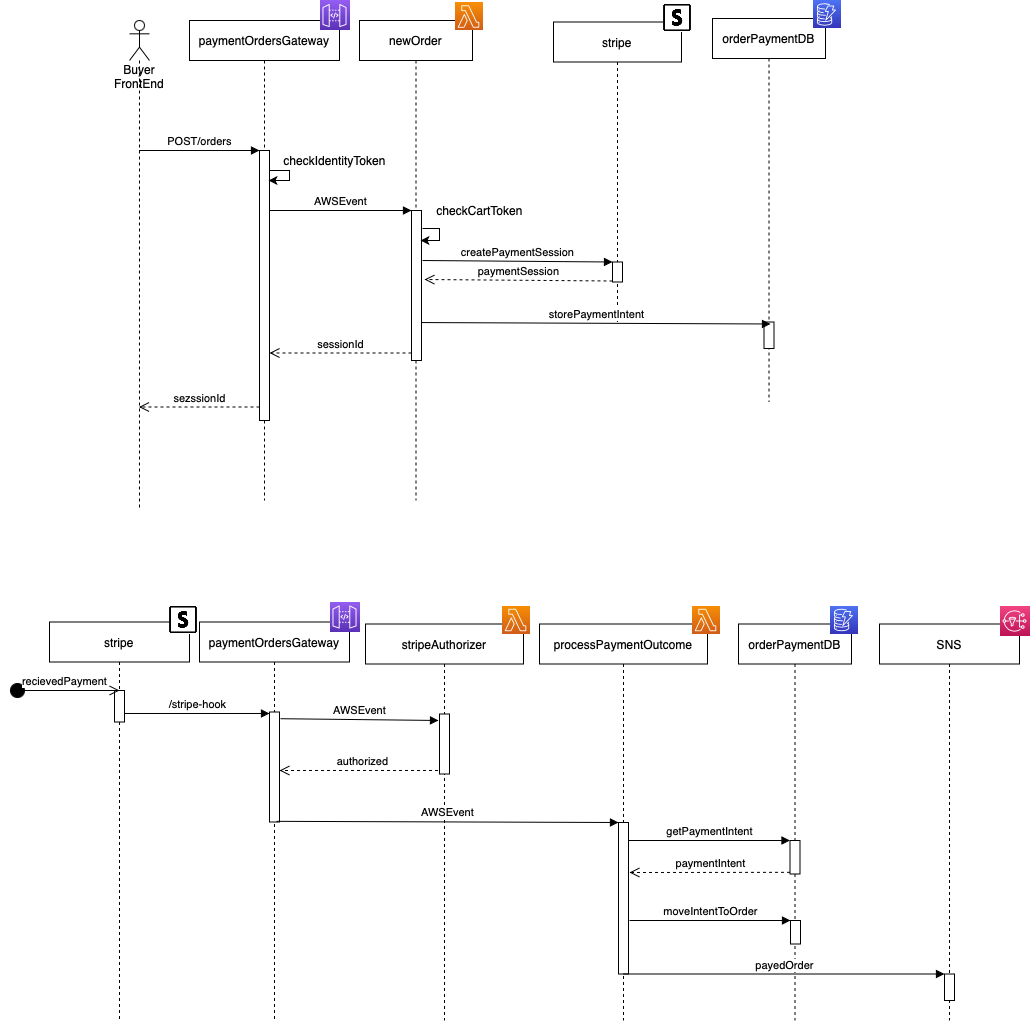
\includegraphics[scale=0.5]{Immagini/Backend/Diagrammiseq.png}
	\caption{Nuovo ordine e pagamento dello stesso}
	\label{fig:Diagrammiseq}
\end{figure}
I precedenti diagrammi rappresentano le tecnologie che entrano in gioco quando l'acquirente della piattaforma effettua un pagamento e, se questo è andato a buon fine, di conseguenza quanto inserito all'interno del carrello verrà trasformato in un'ordine effettuato e di conseguenza visualizzabile dall'utente all'interno dell'elenco degli ordini effettuati.